\subsection{Automating the Scientific Workflow} \label{sec:ai-scientists}

Recent advances in \glspl{gpm}, particularly \glspl{llm}, have enabled initial demonstrations of fully autonomous \gls{ai} scientists \autocite{schmidgall2025agent}. 
We define these as \gls{llm}-powered architectures capable of executing end-to-end research workflows based solely on the final objectives, e.g., \enquote{\textit{Unexplained rise of antimicrobial resistance in Pseudomonas. Formulate hypotheses, design confirmatory in vitro assays, and suggest repurposing candidates for liver-fibrosis drugs}}. 
Such systems navigate partially or entirely through all components of the scientific process outlined in \Cref{fig:applications}, and detailed in the subsequent sections. 

While significant applications emerge in \gls{ml} and programming, scientific implementations remain less explored.

\subsubsection{Coding and ML Applications of AI Scientists}

Notable frameworks, including \modelname{Co-Scientist} \autocite{gottweis2025towards}, and \modelname{\gls{ai}-Scientist} \autocite{yamada2025ai}, aim to automate the entire \gls{ml} research pipeline, typically employing multi-agent architectures (described in detail in \Cref{sec:multi-agent}) where specialized agents manage distinct phases of the scientific method \autocite{schmidgall2025agentrxiv}. 
Critical to these systems is self-reflection \autocite{renze2024self0reflection}---iterative evaluation and criticism of results within validation loops. 
However, comparative analyses reveal that \gls{llm}-based evaluations frequently overscore outputs relative to human assessments \autocite{huang2023mlagentbench0, chan2024mle, starace2025paperbench0}. 
From an engineering perspective, alternative approaches focus specifically on iterative code optimization, enabling systems to refine their codebases \autocite{zhang2025darwin} or generate improved agents autonomously \autocite{hu2024automated}.
In another work, \modelname{AlphaEvolve} \autocite{novikov2025alphaevolve}, which is an \gls{llm} operating within a \gls{ga} environment, found novel algorithms for matrix multiplication (which had seen no innovation in fifty years) and sorting.

\subsubsection{Chemistry and Related Fields}

In chemistry, proposed systems show promising results. \modelname{Robin} identified ripasudil as a treatment for \gls{damd} \autocite{ghareeb2025robin0}---despite pending clinical trials and the general debate for these systems about novelty of their findings\autocite{Listgarten2024perpetual}.
However, automation of experiment execution poses a major constraint for the chemistry-focused \gls{ai}-scientists due to hardware requirements, making computational chemistry the most feasible subfield in which agents have successfully run simple quantum simulations \autocite{Zou2025ElAgente}. 
Further, the \glspl{llm} powering these systems exhibit limited chemical knowledge \autocite{mirza2024large}. 
Despite this, \modelname{ether0} \autocite{narayanan2025training}---the first chemistry-specialized reasoning \gls{llm} (see \Cref{sec:rl} for a deeper discussion on reasoning models)---demonstrated strong capabilities in molecular design and accurate reaction prediction, positioning it as a promising foundation for chemistry-focused \gls{ai} scientists.

\subsubsection{Are these Systems Capable of Real Autonomous Research?}

Although agents like \modelname{Zochi} \autocite{intologyai2025zochi} achieved peer-reviewed publication in top-tier venues (\gls{acl} 2025), their capacity for truly autonomous end-to-end research remains debatable \autocite{son2025ai}. 
Even when generating hypotheses that appear novel and impactful, their execution and reporting of these ideas, as demonstrated by \textcite{si2025ideation1execution}, yield results deemed less attractive than those produced by humans. Additionally, this autonomy raises a critical question: \textit{What should the role of \gls{ai} in science be?} 
While these systems can generate hypotheses, conduct experiments, and produce publication-ready manuscripts, their integration demands careful consideration (refer to \Cref{sec:ethics} for further discussion about moral concerns around these systems). 
Beyond the vision of fully autonomous scientists, \glspl{gpm}---primarily \glspl{llm}---are already utilized across most scientific workflow components, for which \glspl{llm} have proven useful for some. 
These elements are shown in \Cref{fig:applications}, and we discuss next.


\begin{figure}[!ht]
    \centering
    \label{fig:applications}
    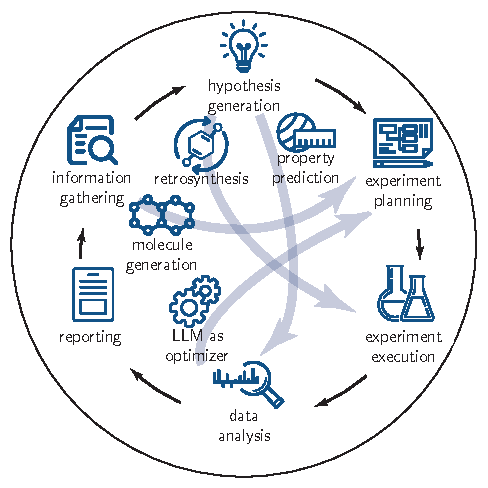
\includegraphics[width=0.5\textwidth]{figures/rescaled_figures/chemrev_figure11.pdf}
    \caption{\textbf{Overview of the scientific process}. The outer elements represent the typical scientific research process: from gathering information and generating hypotheses based on the observations, to executing experiments and analyzing the results. The terms that are in the center represent data-driven \enquote{shortcuts} that \enquote{accelerate} the typical scientific method. All stages represented in the figure are discussed in detail in the following sections.}
\end{figure}